\chapter{Background} \label{chapter:part2-background}
\graphicspath{{Part2/Background/figures/}}

\section{Data Integration}\label{section:dataIntegration}

\textit{Data Integration (DI)} is the process of providing the user with a unified view of data residing at different sources~\cite{Lenzerini:DIT:02}. Data Integration is a challenging task since these sources are in many real-world mutually inconsistent.

Various approaches and methodologies have been proposed to solve the DI problem in the enterprise:
\begin{itemize}
	\item XML as a hierarchical data format can be used as a uniform standard uniform for data representation. However, extending XML to provide complex mappings and sources descriptions is difficult.
	\item SOA can be seen as a holistic approach for distributed systems communication and architecture. In its core, SOA aims at minimizing impedance in the architecture paving the way for easier communication between data sources. However, in~\cite{Frischmuth:ISWC:13}, the authors argue that SOA is well-suited for transaction process rather than an approach for data integration.
	\item Ontologies can be used as a rich format to describe queries and data mappings between schemas and sources. However, developing ontologies require specific skills and it is difficult to provide a complete model that captures the dynamics of the enterprise.
	\item Linked Data paradigm is a slightly different approach from the ontology-based by exploiting Semantic Web technologies like RDF to represent enterprise taxonomies. The LD approach allows terms to be easily reused and extended.
\end{itemize}

\subsection{Data Warehousing (DW)}

A \textit{Data Warehouse (DW)} is a large repository where integrated data from different resources reside for the purpose of analysis. Feeding data into the warehouse is done using the Extract-Transform-Load (ETL) process: First the data is extracted from the operational source systems (ERP, CRM, etc.) and the then the transformation process is applied in order to unify the data into the warehouse format. Finally the loading is process is applied to import the data to the warehouse.

Querying DWs is done by special systems that aggregate measure values over a range of dimension values. One of those systems is the Online Analytical Processing (OLAP). OLAP systems provide fast answers to queries that aggregate large amounts of data to find overall trends; the results are presented in multidimensional fashion. As opposed to the well known Online Analytical Transaction Processing (OLTP) the focus is on data analysis rather than transactions. Moreover, when doing OLTP the focus is on a single transaction whereas OLAP systems keep track of each individual transaction. OLAP systems generally never delete nor update its data; only additions of new data takes place periodically, thus OLAP systems are optimized for retrieving and summarizing large amounts of data.

\section{Business Intelligence}\label{section:businessIntelligence}

\textit{Business Intelligence (BI)} is the set of techniques and tools for transforming raw data into meaningful and useful information to be used in the decision making process~\cite{Rud:Wiley:09}. BI consists of various number of components including Data Integration, Data Quality and Data Warehousing among others.

\subsection{Multidimensional Model}

Traditional relational model is efficient in performing "online" transactions. However, it had clear shortcomings when the objective was to analyze large scale data. The multidimensional model was designed specifically to support data analysis by presenting data as facts with associated numerical values. The multidimensional model has the following fundamental concepts:

\begin{itemize}
	\item \textbf{Dimensions}: Textual data used for labeling, selection, filtering and grouping of data at various levels of details. A dimension is organized into a containment-like hierarchy composed of number of levels, each of which represents a specific level of details. The instances of the dimensions are typically called dimension values or members; each value or member belongs to a particular level.

\begin{figure}[htbp]
\centering
	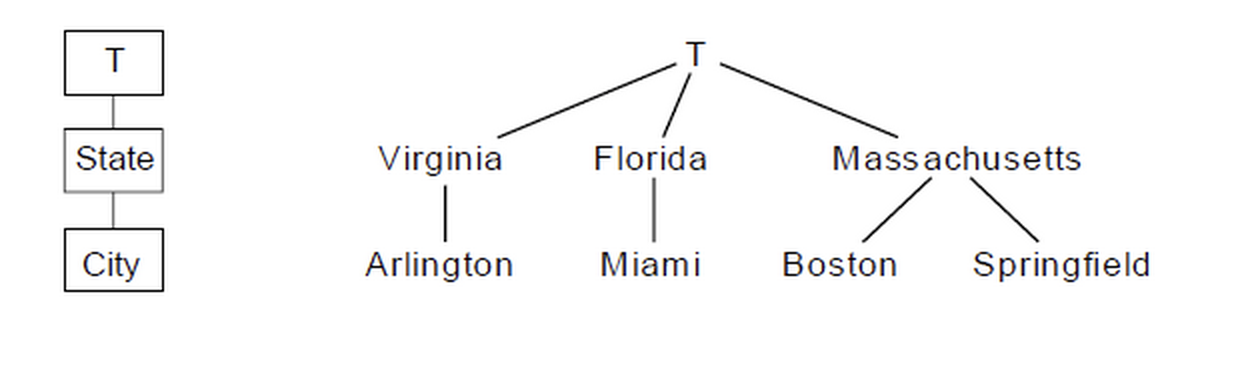
\includegraphics[width=\linewidth]{dimension.png}
	\caption{Example of a hierarchical geography dimension}
	\label{fig:dimension}
\end{figure}

	\item \textbf{Measures}: A measure has two components, a numerical property and a formula (usually an aggregation function such as sum or average). Measures generally represent the properties of a chosen fact.
	\item \textbf{Facts}: Facts are the objects that present the subject of the analysis. They are mostly defined by their combination of dimension values. a fact has a certain granularity which is determined by the levels from which its dimension values are drawn.
	\item \textbf{Cubes}: A cube is a multidimensional data structure for capturing and analyzing data. It generalizes the tabular spreadsheet such as there can be any number of dimensions (in contrast to only two in the tabular spreadsheets).
\end{itemize}

\subsection{SAP BI Application Suite}

The SAP BI application suite can be divided into the following main areas:

\begin{itemize}
	\item \textbf{Analysis Solutions}: Empower analysts with the ability to analyze multidimensional data and quickly answer sophisticated business questions.
	\item \textbf{Discovery Solutions}: Provide an interface to access, transform and visualize data in a self-serviced way.
	\item \textbf{Predictive Solutions}: Provide intuitive and easy-to-use environment to design and visualize complex predictive models.
	\item \textbf{Dashboard Solutions}: Allow creation of rich Visualizations that allow users interaction with their data. SAP Lumira which is used by our analyst \textbf{Bob} is part of these solutions.
	\item \textbf{Reporting Solutions}: Offers powerful interfaces that enable analysts and non-technical users to ask spontaneous and iterative business questions about their data.
\end{itemize}

\section{SAP High Performance Analytic Appliance (HANA)}

SAP High Performance Analytic Appliance (HANA)\footnote{\url{http://hana.sap.com/}} is an in-memory data platform that is deployable as an on-premise appliance, or in the cloud. It is a revolutionary platform that is best suited for performing real-time analytics, and developing and deploying real-time applications. At the core of this real-time data platform is the SAP HANA database which is fundamentally different than any other database engine in the market today. It leverages the cheap price of memory chips and does the computation operations all in the memory instead of disk. For BI and Real-time analytics HANA specializes on:

\begin{itemize}
	\item \textbf{Data Warehousing}
	\item \textbf{Operational Reporting}: Provides real-time insights from transaction systems such as ERP.
	\item \textbf{Predictive and Text analysis on Big Data}: Provides the ability to perform predictive and text analysis on large volumes of data in real-time. It does this through the power of its in-database predictive algorithms and its R integration capability. With its text search/analysis capabilities SAP HANA also provides a robust way to leverage unstructured data.
\end{itemize}

\begin{figure}[ht]
\centering
	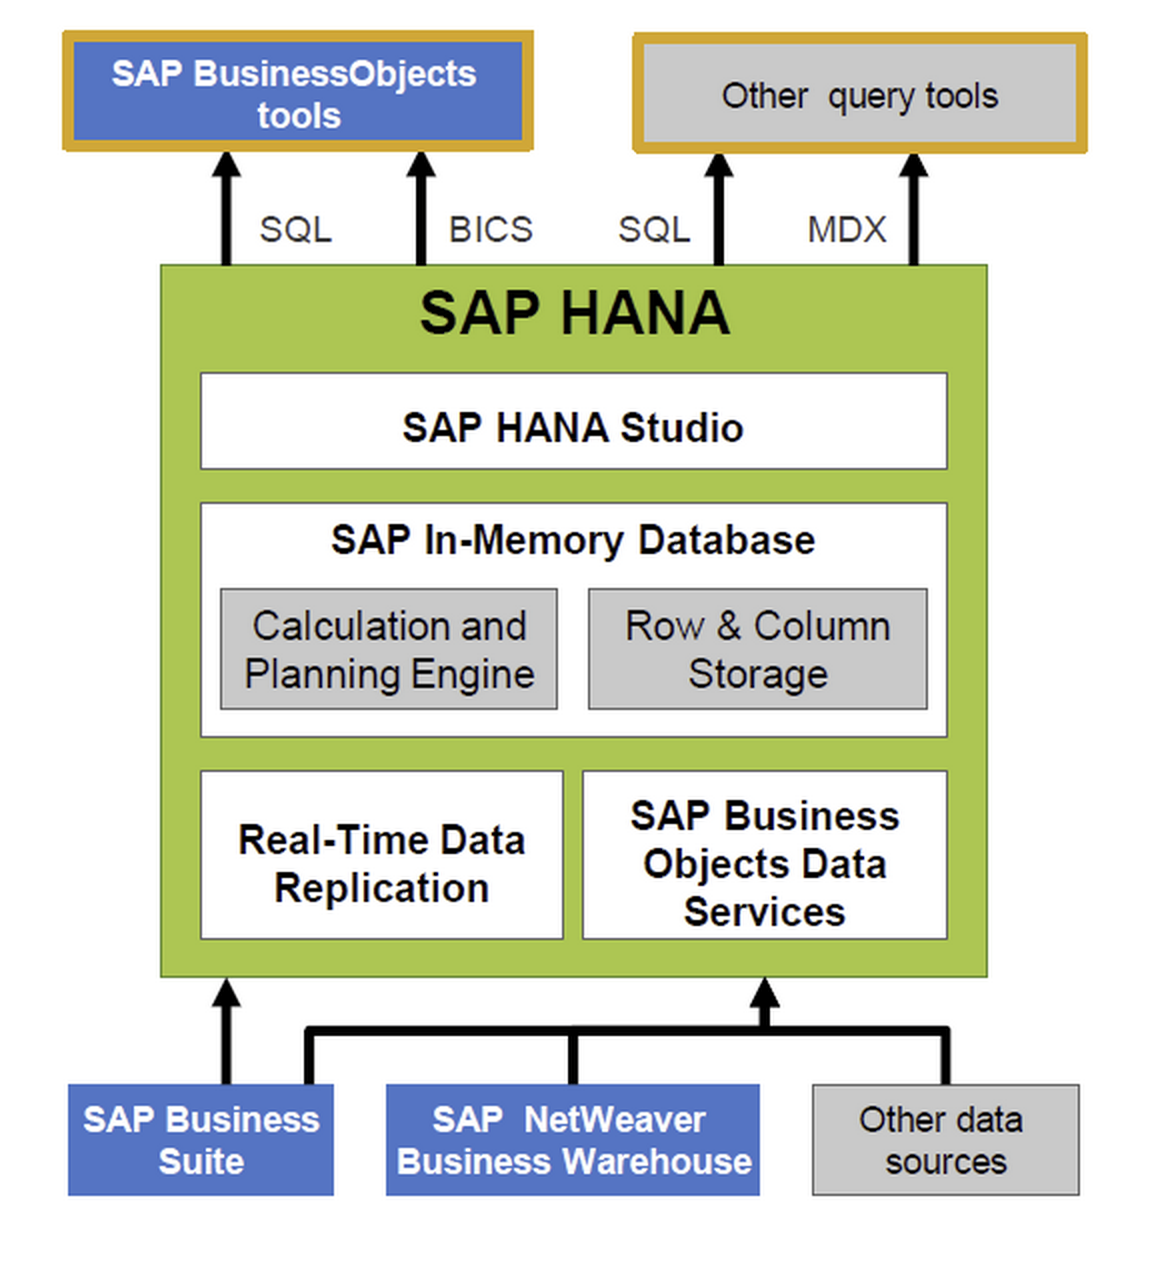
\includegraphics[scale=0.5]{hana_architecture.png}
	\caption{SAP's High Performance Analytic Appliance (HANA) in SAP BI suite}
	\label{fig:hana_architecture}
\end{figure}

HANA has both columns and rows stores for data storage, the user specifies on which data store he wishes to put his data; row stores are fit for traditional transaction systems (traditional databases) when transactions are done on row level; however BI queries or analytical queries are done on subsets of columns; so the database does not need to access all the elements in a row in order to fetch the required data.

HANA has mainly three views on data:

\begin{itemize}
	\item \textbf{Attribute Views}: Used to model dimensions and perform all types of joins. In most cases used to model master data like entities (like Product, Location, Business Partner). For example; If i have my product details scattered in more than one table; but i need to model my product as one business entity; i need to create an attribute view that aggregates data from different tables into one single entity which is product.
	\item \textbf{Analytical Views}: Used for calculation and aggregation. Adds transactional tables and measures (key figures), calculates aggregates (e.g. No. of Products sold per year), joins Attribute Views. It is defined at least on one fact table. In most cases used for exposing transactional data by joining the fact table with Attribute Views.
	\item \textbf{Calculation Views}: Performs complex Views calculations not possible with other views and uses SQLScript.
\end{itemize}

\subsection{HANA XS-Engine}

Consuming data from HANA needs a lot of pre-configuration; to ease this process the XS-Engine was created to act as Lightweight Application Server within HANA DB; its a presentation logic on client sides that encapsulated control flow logic and calculation logic providing REST and ODATA interfaces.

\subsection{Active Information Store (AIS)} \label{ais}

The Active Information Store (AIS) is a graph engine built on top of HANA. AIS provides storage and query services on graphs. AIS offers a flexible data representation model (see figure~\ref{fig:ais}) that contains:

\begin{figure}[htbp]
\centering
	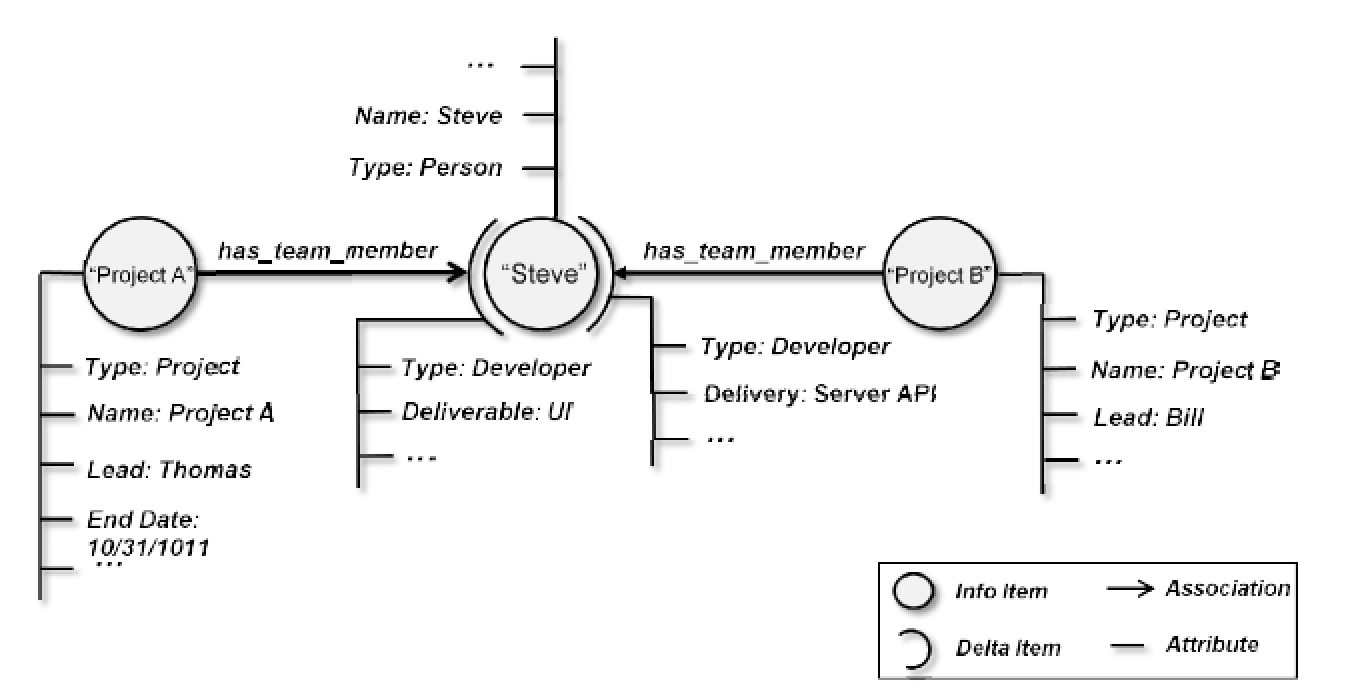
\includegraphics[scale=0.5]{ais_model.png}
	\caption{AIS data model}
	\label{fig:ais}
\end{figure}

\begin{itemize}
	\item \textbf{Info Items}: They are the vertices in the graph. They represent a unique single identifiable data instance. Info Items can have a set of properties that describe them. Each Info Item is identified by its URI and must belong to at least one workspace. A Workspace establishes a scope for visibility and access control.
	\item \textbf{Associations}: They are the edges in the graph. Associations can further have attributes which describe them.
	\item \textbf{Attributes}: Typed properties used to describe Info Items and Associations.
\end{itemize}

\section{Social Web}\label{social-web}

The social web (Web 2.0) is about websites and services designed and developed to support and foster social interactions~\cite{Porter:NewRiders:08}. The social web spans services like blogs, wikis, crowdsourcing and social media services. These services are often accompanied with APIs that allow rapid community driven expansion of complementary services. In this thesis, we use the following popular social media services:

\begin{itemize}
	\item \textbf{Twitter}\footnote{\url{http://twitter.com}}: A service allowing users to send rich short messages of 140 characters called "tweets" or "microposts". Twitter allow users to "follow" each other and start private conversations. Users can interact with tweets by replying or forwarding (re-tweeting) them. Tweets can contain multimedia parts like photos or videos and can be tagged with certain keywords preceded by the hash character called "hashtags" e.g. \#tag.
	\item \textbf{Google+}\footnote{\url{https://plus.google.com}}: A social media service owned by Google focusing on driving interest-based conversations and interactions. In its core, Google+ evolves around the concept of "circles" which enable users organize people into groups or lists. Similarly to Twitter, posts can be tagged with hash-tags entered manually by users or added automatically by Google+.
	\item \textbf{Stack Exchange}\footnote{\url{http://stackexchange.com}}: A question and answer group of websites. Each website specializes in a topic like technology, politics, food, etc. Users are encouraged to provide answers and helpful comments by providing a reputation award system allowing the content to be self-moderating.
	\item \textbf{YouTube}\footnote{\url{http://youtube.com}}: A video sharing website owned by Google. The site allows users to upload, view and share videos. Moreover, YouTube allows live streaming of events with the ability to interact with the video feed through comments.
	\item \textbf{Vimeo}\footnote{\url{http://vimeo.com}}: Another video sharing website with a more focused community of professionals in various areas than YouTube.
	\item \textbf{Slideshare}\footnote{\url{http://slideshare.com}}: A slide hosting service where users can upload their presentations in various formats to be viewed and shared on the website. The website also supports documents, videos and webinars and acts as an educational and e-learning hub.
\end{itemize}

